\section{Design and Implementation}
\subsection{DeAr Micro-architecture Design}
Fig.~\ref{fig:micro} illustrates the micro-architecture of DeAr.
Two DeAr threads share the ALU that commonly exist in a RISC datapath.
The demonstrated example includes an adder, a multiplier and a barrel shifter, which are qualified to perform most benchmarks.
The output of each arithmetic unit contains an accumulator latch preserving and forwarding the arithmetic result.
The forwarding mechanism and resolution of structural hazards are both handled by the HDFG-based scheduling.
\\\indent
The RF is physically and symmetrically separated for two threads.
Each thread owns a pair of queue memory as well as a stack memory, 
and these memory modules form the sequential-accessed banked register file (SBRF).
A load-queue and a store-queue serve as the buffer that connects the lower level of the memory hierarchy with the datapath.
They can be accessed from their both sides concurrently in the first-in-first-out (FIFO) fashion.
By preventing queues from empty or full with clever scheduling, the latency of load/store can thus be hidden.
The stack memory, on the other hand, is responsible for the storage of intermediate data.
Any access to the SBRF are simplified to "PUSH" or "POP" instead of conventional random-access.
Such an implicit access mechanism reduces both the code size and decode complexity, 
and constitutes the crucial advantage of DeAr over conventional architectures.
\\\indent
The design of transport triggered data bus (TTDB) was inspired by TTA~\cite{tta}.
TTDB separates the RF from ALU with a set of multiplexers controlled by the instruction unit, 
and forwards data from accumulators to ALU inputs.
It is important to note that, even though the communication among the RF, ALU and accumulators is compacted exhaustively, 
the datapath flexibility is still kept.%
\begin{figure}[t]
    \centering
    \includegraphics[width=0.33\textwidth]{./figs/micro.eps}
    \caption{Micro-architecture of a DeAr DSP lane}
    \label{fig:micro}
\end{figure}
\subsection{Data Flow Graph to Hierarchical Data Flow Graph}
\label{sec:hdfg}
A data flow graph (DFG), shown in Fig.~\ref{fig:dfg:dfg}, presents dependencies among operations of a program.
We express a DFG with the data structure, $G$, which holds an operation set $V_{op}$ and a dependency set $E_{op}$.
In conventional DSP, scheduling is usually accomplished based on the DFG analysis.
\\\indent
To go beyond DFGs, we propose the hierarchical data flow graph (HDFG).
Fig.~\ref{fig:dfg:hdfg} demonstrates a HDFG, $\bar{G} = (V_{bt}, E_{bt})$, converted from Fig.~\ref{fig:dfg:dfg}.
Properties of HDFGs include: 
\textbf{(1)} Cascaded operations ($op$) form a super node ($sn$), and an isolated $op$ forms a $sn$ directly. 
Within a $sn$, an $op$ forwards data to the next one.
\textbf{(2)} Neighboring $sn$s form a full binary tree ($bt$), and isolated $sn$ forms a $bt$ directly.
These $bt$s further form a set of vertices, $V_{bt}$.
Within a $bt$, a parent $sn$ receives the first operand popped from the stack and the second one forwarded via TTDB.
\textbf{(3)} Dependencies among $op$s that cross $bt$s are inherited by the $bt$s they belong to.
These inherited dependencies form a set of edges, $E_{bt}$, of $V_{bt}$.
\textbf{(4)} A $bt$ without any in-edge existing in $\bar{G}$ (i.e., $bt \in V_{bt}\ |\ \textrm{deg}^-(bt) = 0$) is free to be scheduled. 
After scheduled, the $bt$ and its edges are erased from the $\bar{G}$.%
\setlength{\textfloatsep}{10pt}% Remove \textfloatsep
\begin{figure}[t]
\begin{center}
\subfigure[DFG example]
{
\label{fig:dfg:dfg}
\includegraphics[width=0.19\textwidth]{figs/dfg.eps}
}%
\hspace{0.5em}
\subfigure[Corresponding HDFG]
{
\label{fig:dfg:hdfg}
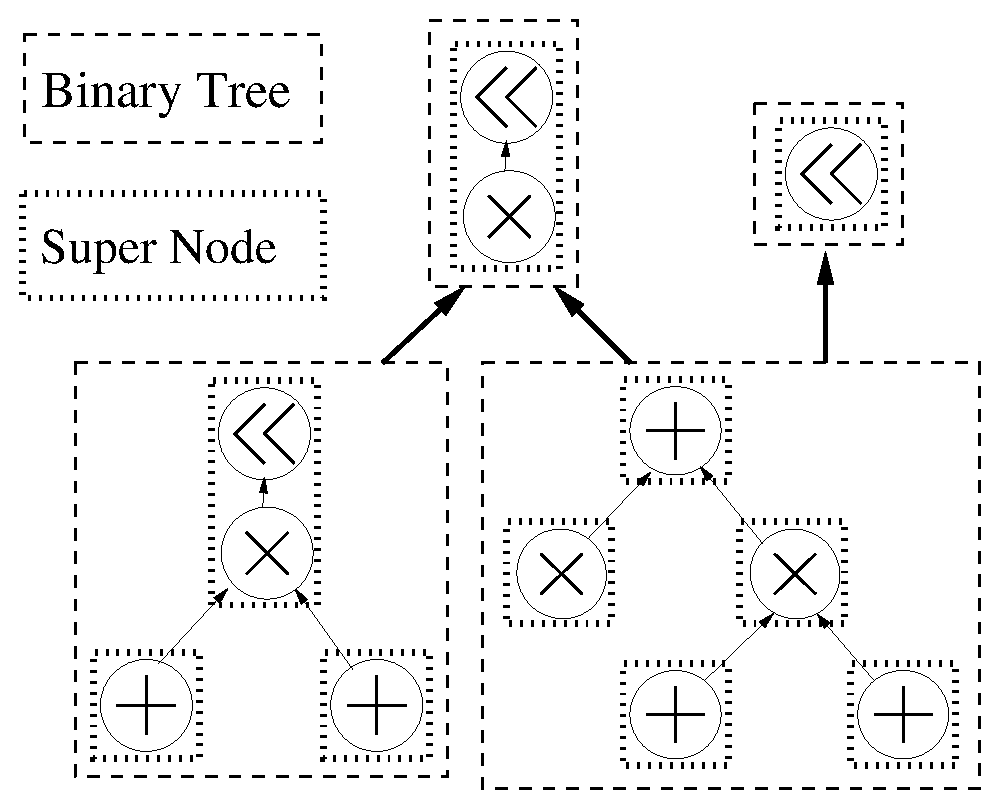
\includegraphics[width=0.21\textwidth]{figs/hdfg.eps}
}
\end{center}
\caption{Conversion from DFG to HDFG}
\label{fig:dfg}
\end{figure}
\subsection{HDFG-based Scheduling}
\label{sec:scheduling}
The goal of the DeAr scheduler is generating the binary code with maximum ILP, maximum data forwarding rate, 
and minimum stack memory consumption of each thread.
To achieve the goal, we present a novel scheduling algorithm, 
\textproc{HDFG-based scheduling}, which is shown in Algorithm~\ref{alg}.
The algorithm takes an HDFG ($\bar{G}$) as the input and generates the output binary code ($X_{final}$).
\\\indent
The scheduler firstly completes the \textit{Inter-tree scheduling phase}
for the purpose of dispatching operations from independent $bt$s to two threads.
Line~\ref{line:interws}--\ref{line:interwe}, enclosed by a while loop, is the \textit{Inter-tree scheduling phase}, 
where the scheduler performs symmetric steps for two threads.
If there is a thread with an empty operation-list, 
the scheduler searches $\bar{G}$ and selects a free $bt$ randomly, 
and assigns operations in the $bt$ sorted by higher-subtree-first postorder-traversal (\textproc{HFPT Sort}) to its operation-list.
The postorder-traversal ensures that children are listed in front of their parent, 
and the higher-subtree-first policy ensures that nodes of the higher subtree are listed in front of ones of its sibling, 
which minimizes the stack memory consumption.
Next, it performs \textproc{ALU Allocation} for two operation-lists.
This subroutine dispatches operations allowed to execute concurrently, 
and generates the code segment containing the dispatched operations and control signal for SBRF and TTDB.
It applies Dynamic Programming (DP)~\cite{dp} to determine which thread should stall when the ALU conflict occurs.
After \textproc{ALU Allocation}, at least one operation-list is consumed, 
and the returned code segment is accumulated with the current segment.
As shown in Line~\ref{line:intercon}, we use $\oplus$ to denote the code accumulation.
The loop proceeds until all $bt$s in $\bar{G}$ are scheduled.
\\\indent
Nevertheless, it is very likely that one of operation-lists has operations remaining at the last iteration.
Line~\ref{line:interis}--\ref{line:interie} illustrate such a scenario.
Remaining operations are thus reverted to the original form of $bt$ by the subroutine \textproc{Restore Subtree from list},
and a remaining subtree, $bt_{remain}$, is obtained.%
\\\indent
To deal with the $bt_{remain}$, 
the scheduler performs the \textit{Intra-tree scheduling phase}, 
which dispatches operations from two subtrees of the $bt_{remain}$ to two threads respectively.
Line~\ref{line:intra:ws}--\ref{line:intra:we} show a while loop for \textit{Intra-tree scheduling phase}.
A crucial strategy applied here is, partitioning $bt_{remain}$ into three parts:
the root node, left and right subtrees.
Since operations in the root must be handled sequentially, 
we can dispatch them directly with a single thread (thread 1), 
and obtain a binary code segment, $X_{single}$.
Then, by treating the left and right subtrees as independent trees, 
we can perform similar steps applied in the \textit{Inter-tree scheduling phase}.
We manipulate \textproc{HFPT Sort} and \textproc{ALU Allocation} again, and obtain another binary code segment, $X_{intra}$.
By repeating above steps, $bt_{remain}$ keeps shrinking while $X_{intra}$ and $X_{single}$ keep accumulating,
until all operations left in $bt_{remain}$ are dispatched.
Finally, we concatenate $X_{inter}$, $X_{intra}$ and $X_{single}$,
and obtain the complete code $X_{final}$.
%-----------Inter-tree-------------
%\setlength{\textfloatsep}{0pt}% Remove \textfloatsep
\begin{algorithm}[t]
{
        \fontsize{8pt}{9pt}\selectfont
    \caption{\textproc{HDFG-based Scheduling}}
    \begin{algorithmic}[1]
        \Require    HDFG $\bar{G} = (V_{bt}, E_{bt})$
        \Ensure     $X_{final}$
        \State $X_{inter},X_{intra},X_{single}\Leftarrow NULL$       %\Comment{Initialize $X_{inter}$}
        \While{$V_{bt} \neq \emptyset$} \label{line:interws}
        \Comment \textit{Inter-tree scheduling phase}
        \If{$op\_list_{thread1} = \emptyset$}
        %\State Select $bt \ni \sum_{bt \in V_{bt}}\textrm{deg}^-(bt) = 0$
        \State $op\_list_{thread1} \Leftarrow$ \Call{HFPT Sort }{$bt$}, where $bt\in V_{bt}\ |\ \textrm{deg}^-(bt) = 0$ 
        %\State Erase $bt$ and its edges from $\bar{G}$
        \EndIf
        \If{$op\_list_{thread2} = \emptyset$}
        \State $op\_list_{thread2} \Leftarrow$ \Call{HFPT Sort }{$bt$}, where $bt\in V_{bt}\ |\ \textrm{deg}^-(bt) = 0$
        %\State Erase $bt$ and its edges from $\bar{G}$
        \EndIf
        \State $X_{1} \Leftarrow X_{1}\oplus$\Call{ALU Alloc}{$op\_list_{thread1}$,$op\_list_{thread2}$} \label{line:intercon}
        \EndWhile \label{line:interwe}
        \If{$work\_queue_{thread1} \neq \emptyset$} \label{line:interis}
        \State $bt_{remain} \Leftarrow$ \Call{Restore-Subtree}{$op\_list_{thread1}$}
        \State Clear $work\_queue_{thread1}$
        \ElsIf{$work\_queue_{thread2} \neq \emptyset$}
        \State $bt_{remain} \Leftarrow$ \Call{Restore-Subtree}{$op\_list_{thread2}$}
        \State Clear $work\_queue_{thread2}$
        \Else
        \State $bt_{remain} \Leftarrow NULL$
        \EndIf \label{line:interie}
        \While{$bt_{remain} \neq \emptyset$}    \label{line:intra:ws}
        \Comment \textit{Intra-tree scheduling phase}
        \State $X_{single} \Leftarrow$ \Call{Gen Code Single Thread }{$bt_{root}$} $\oplus X_{single}$
        \State $op\_list_{thread1} \Leftarrow$ \Call{HFPT Sort }{$bt_{left-subtree}$}
        \State $op\_list_{thread2} \Leftarrow$ \Call{HFPT Sort }{$bt_{right-subtree}$}
        \State $X_{body} \Leftarrow X_{body} \oplus$ \Call{ALU Alloc }{$op\_list_{thread1}$, $op\_list_{thread2}$}
        \If{$work\_queue_{thread1} \neq \emptyset$}
        \State $bt_{remain} \Leftarrow$ \Call{Restore Subtree}{$work\_queue_{thread1}$}
        \State Clear $work\_queue_{thread1}$
        \ElsIf{$work\_queue_{thread2} \neq \emptyset$}
        \State $bt_{remain} \Leftarrow$ \Call{Restore Subtree}{$work\_queue_{thread2}$}
        \State Clear $work\_queue_{thread2}$
        \Else
        \State $bt_{remain} \Leftarrow NULL$
        \EndIf
        \EndWhile   \label{line:intra:we}
        \State $X_{final} \Leftarrow X_{inter} \oplus X_{intra} \oplus X_{single}$
        \State \Return{$X_{final}$}
    \end{algorithmic}%
    \label{alg}
}
\end{algorithm}

